\chapter{Clusterização como um serviço} \label{cap:api}

  Uma solução para atender as necessidades do ``Empurrando Juntos'' é oferecer
  o processo de clusterização, juntamente com as funcionalidades de gerenciamento
  de conversas, comentários e votos, como um serviço.
  Uma forma de conseguir essa integração com o ``Empurrando Juntos'' é oferecer
  esses serviços através de uma \textit{Application Programming Interface} (API).

  De acordo com \citeonline{understanding_web}, uma API é uma interface que permite que os 
  usuários interajam ou respondam a dados ou serviços solicitados de outro programa, outros
  aplicativos ou sites. No contexto da Web, as APIs facilitam a troca de dados entre 
  aplicações, permitem a criação de novas aplicações e constituem a base para o conceito de 
  ``Web como uma plataforma''.

  \citeonline{wagh2012comparative} afirmam que existem vários métodos para interação entre o  
  usuário e a Internet, através de serviços web (web \textit{services}).
  Essa arquitetura permite que os componentes de software, o que inclui funções,
  objetos e processos de diferentes sistemas, sejam expostos como um serviço.

  Para prover esses serviços através de uma API, o estilo arquitetural Transferência de Estado 
  Representacional (do inglês, \textit{Representational State Transfer} ou REST)
  se destaca atualmente como representante do provimento de serviços via \textit{Web} e, portanto, foi escolhido para
  guiar a implementação da API proposta.

  O estilo REST é um estilo arquitetural introduzido por \citeonline{fielding2002} que serve como um modelo abstrato
  para guiar o uso do \textit{Hypertext Transfer Protocol} (HTTP) e do \textit{Uniform Resource Identifier} (URI)
  na arquitetura da Web moderna, abstraindo os elementos arquiteturais participantes de um sistema de
  hipermídia distribuído.
  O REST é um conjunto coordenado de restrições arquiteturais que possibilita 
  baixo acoplamento entre os componentes e minimização da latência da comunicação e que
  favorece a escalabilidade da implementação dos componentes \cite{fielding2002}.
  
%   \citeonline{perry1992} classificam os elementos arquiteturais em elementos de processamento (componentes),
%   elementos de dados e elementos de conexão (conectores). O estilo REST foca no papel dos componentes, nas restrições
%   da interação entre componentes e na interpretação de elementos de dados significantes para a interação \cite{fielding2002}.
  
  No estilo REST, uma informação é abstraída em um recurso, que pode ser qualquer informação que possa ser nomeada
  (documentos, imagens, serviços, entre outros). Para identificar um recurso específico na interação entre dois
  componentes, o REST utiliza um identificador de recurso (URI) \cite{fielding2002}.
  
  Componentes REST se comunicam transferindo uma representação do dado (informação) em algum formato padrão que pode
  ser selecionado dinamicamente com base nas preferências do destinatário \cite{fielding2002}. Além dos dados contidos na 
  informação, uma representação contém também metadados descrevendo os dados e, possivelmente, metadados sobre os
  metadados \cite{fielding2002}.
  
      \citeonline{richardson09} propôs um modelo de maturidade para classificar
      APIs RESTful de acordo com os mecanismos da \textit{web} utilizados,
      que foi explicado de uma forma mais simples por \citeonline{fowler10}.
      A Figura \ref{fig:glory_of_rest}, apresentada por \citeonline{fowler10},
      ilustra os níveis do modelo de maturidade de \citeonline{richardson09}.
	
      \begin{figure}[h!]
	\centering
	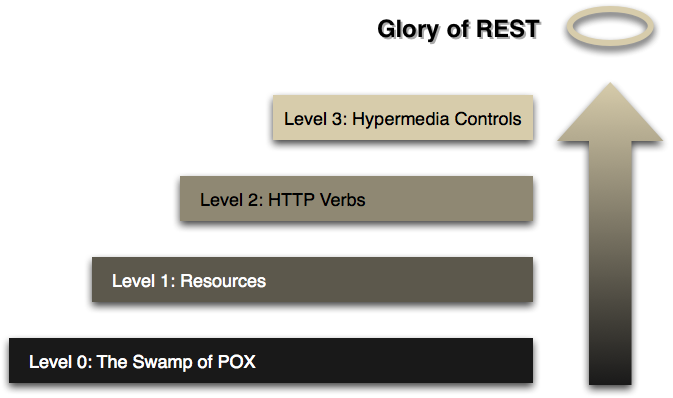
\includegraphics[scale=0.5]{figuras/glory_of_rest.png}
	\caption{Níveis do modelo de maturidade proposto por Richardson. Fonte: Traduzido de \cite{fowler10}}
	\label{fig:glory_of_rest}
      \end{figure}
      
      O nível zero consiste em utilizar o procotolo HTTP apenas como um meio de transporte de mensagens,
      comumente utilizando apenas um verbo HTTP (GET, POST e etc) e apenas um URI como ponto de entrada da API, 
      usando o HTTP com um túnel para uma comunicação remota \cite{fowler10} \cite{richardson09}.
      Essa característica é presenciada em APIs que implementam o protocolo \textit{Simple Object Access Protocol} (SOAP).
      
      O primeiro nível é alcançado quando se introduz o uso de recursos na API,
      o que permite identificar recursos individuais por meio URIs únicas,
      fornecendo pontos de entrada mais coesos para a API \cite{fowler10} \cite{richardson09}.
      
      O segundo nível é atingido quando a API utiliza da forma mais semântica possível
      os verbos e códigos de respostas providos pelo protocolo HTTP,
      fornecendo entradas e respostas mais semanticamente corretas \cite{fowler10} \cite{richardson09}.
      
      O terceiro e último nível é alcançado quando controles de hipermídia
      são introduzidos nas respostas da API \cite{fowler10} \cite{richardson09}.
      Este último nível, conhecido como ``Glória do REST'' por \citeonline{fowler10},
      refere-se à restrição \textit{Hypertext As The Engine Of Application State} (HATEOAS) 
      que fornece meios (\textit{hyperlinks}) para informar ao cliente o que pode ser feito em seguida,
      para que ele possa navegar nos \textit{endpoints} da API de forma mais simples.
      
  A criação de uma API RESTful para o contexto deste trabalho é adequada, pois promove baixo acoplamento
  entre os componentes da aplicação, não sobrecarregando o ``Empurrando Juntos'' com funcionalidades genéricas
  para as conversas e de agrupamento dos usuários,
  permitindo a reutilização dos serviços de clusterização por qualquer
  outra aplicação que já existe ou que venha a ser criada, tanto \textit{web} como \textit{mobile}.
  
\section{Arquitetura da solução} \label{architecture}
    
    Considerando o objetivo do trabalho de implementar uma API capaz de trabalhar com 
    módulos matemáticos plugáveis, a solução proposta está representada na Figura \ref{fig:pentano}, 
    na qual são indicados os dois módulos tratados na solução: os módulos API e Matemático. 
    A API implementada neste trabalho em conjunto com uma aplicação cliente a ser implementada em outro momento,
    será denominado neste trabalho de \textit{Pentano}\footnote{Nome da proposta no trabalho de \citeonline{tallys_tcc}}.
    
    \begin{figure}[h!]
    \centering
    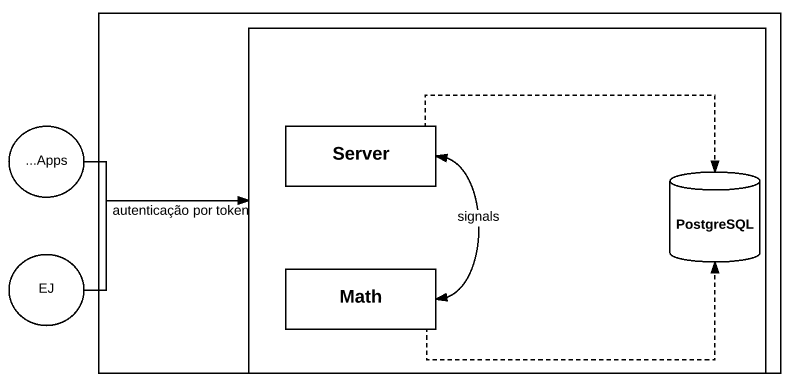
\includegraphics[scale=0.7]{figuras/esquema_pentano.png}
    \caption{Estrutura do Pentano}
    \label{fig:pentano}
    \end{figure}
    
    A arquitetura proposta é definida pelo módulo de API, o módulo Matemático
    e o protocolo de comunicação entre esses dois módulos, como ilustra a Figura \ref{fig:pentano}. O módulo de 
    API é uma aplicação independente que contém a lógica para o gerenciamento das conversas e usuários e
    serve como ponto de entrada para o sistema. Os módulos matemáticos também são aplicações independentes que implementam a 
    interface definida no protocolo
    para se comunicarem com a API, de modo que seja possível criar vários módulos matemáticos utilizando algoritmos diferentes.
    Os módulos matemáticos encapsulam a lógica de agrupar os usuários com base nos votos obtidos.
    
    Como mencionado, para a comunicação entre a API e os módulos matemáticos escolhidos,
    foi utilizado o Celery como plataforma de execução de tarefas assíncronas.
    O Celery funciona a partir da definição de tarefas que podem ser executadas de forma assíncrona
    e utiliza um \textit{message broker}, que é uma plataforma intermediária
    entre duas aplicações para troca de mensagens, para enfileirar e delegar as tarefas para execução.
    
    Essa ferramenta em conjunto com uma interface de tarefas definidas formam
    a comunicação entre a API e o módulo responsável pela clusterização. 
    Uma visão geral do protocolo pode ser vista na Figura \ref{fig:protocolo}.
    

    \begin{figure}[bt!]
    \centering
    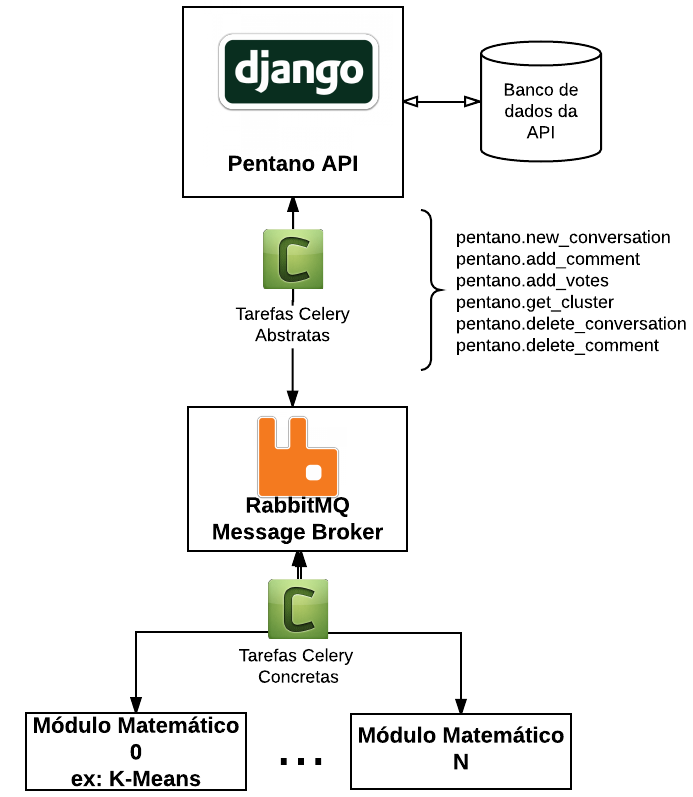
\includegraphics[scale=1]{figuras/esquema_protocolo.png}
    \caption{Esquema de comunicação entre os módulos de API e Matemático}
    \label{fig:protocolo}
    \end{figure}
    
%     Fica a cargo da implantação do sistema de associar a API desenvolvida neste trabalho com algum módulo matemático 
%     existente ou novo.
    
    \subsection{Módulo de API}

	O módulo de API é responsável por gerenciar as conversas, comentários, votos
	e cuidar de todos os aspectos da autenticação das aplicações. Dessa forma, foram mapeadas as entidades principais e 
	os relacionamentos entre elas. 
	As principais entidades que foram identificadas são Usuário, Conversa e Comentário. Um usuário pode criar
	conversas e comentários para cada conversa e participar de outras conversas, criadas por outros usuários.
	A participação de um usuário em uma conversa é dada pelo ato de criação de comentários naquela conversa ou
	no ato de votar em um comentário de uma conversa. Esse mapeamento é ilustrado na Figura \ref{fig:entidades}.

	\begin{figure}[h!]
	\centering
	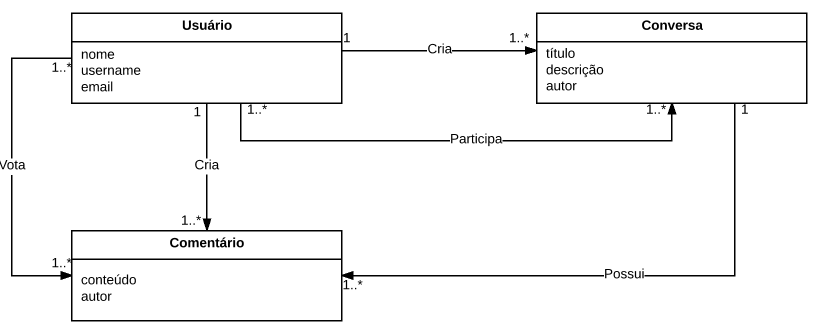
\includegraphics[scale=0.5]{figuras/entidades.png}
	\caption{Relacionamento das principais entidades da API}
	\label{fig:entidades}
	\end{figure}

	Como o \textit{framework} Django foi escolhido como tecnologia de implementação da API,
	a arquitetura proposta foi pensada valendo-se de 
	recursos providos pela própria arquitetura do \textit{framework}.
	No Django, uma aplicação web é abstraída como um projeto, e um projeto é composto por uma coleção de aplicações
	(ou, de forma abreviada, \textit{apps}) independentes, que
	são pacotes Python que proveem um conjunto de funcionalidades relacionadas e podem ser reutilizados \cite{django_apps}.

	Portanto, toda a solução foi componentizada utilizando \textit{apps} do 
	Django. Considerando os requisitos funcionais e não funcionais da solução, especificados anteriormente, a arquitetura da solução foi definida 
	conforme a Figura \ref{fig:arquitetura_api}, onde no módulo \textit{API} temos dois \textit{apps} independentes, um responsável
	por cuidar de toda parte de autenticação da aplicação (\textit{app} de contas) e o outro para gerenciar as entidades de Conversas 
	e Comentário apresentadas na Figura \ref{fig:entidades}. 

	\begin{figure}[h!]
	\centering
	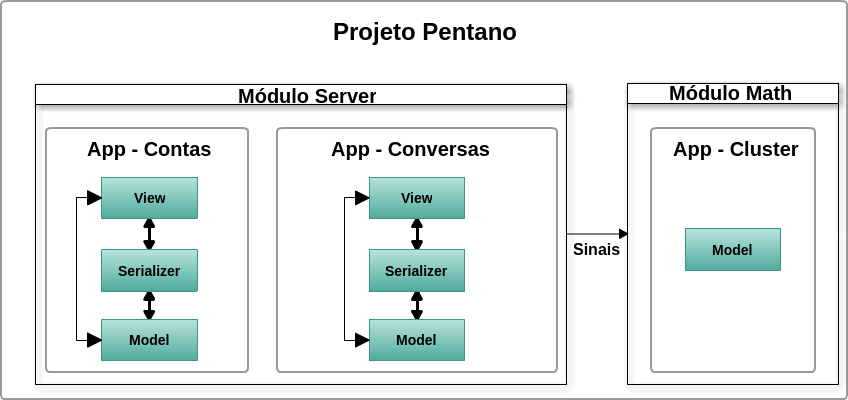
\includegraphics[scale=0.8]{figuras/arquitetura_api.png}
	\caption{Arquitetura de \textit{apps} da API}
	\label{fig:arquitetura_api}
	\end{figure}

	Para cada \textit{app} foi definida uma arquitetura
	em 3 camadas: \textit{models}, \textit{views} e \textit{serializers}.
	A camada \textit{view} recebe e responde as requisições provenientes do cliente.
	A camada \textit{serializer} é responsável pelo tratamento e formatação dos dados das \textit{models}
	para renderização em JSON, seguindo a especificação JSON API.
	Por fim, a camada \textit{model} contém aspectos negociais relacionados a cada uma das entidades definidas na 
	Figura \ref{fig:entidades}.
	
	Para não acoplar as \textit{models} comunicando diretamente com o módulo matemático,
	a comunicação é feita a partir de uma camada de sinais, que são acionados quando alguma ação ocorre nas \textit{models}.
	Esta camada de sinais é implementada utilizando a arquitetura de sinais do Django.
	As seguintes ações possuem sinais registrados:
	
	\begin{itemize}
	 \item Criação de uma nova conversa;
	 \item Criação de um novo comentário;
	 \item Novos votos em um comentário de uma conversa.
	\end{itemize}

    
%     \vfill
%     \pagebreak
    
    \subsection{Módulo matemático}
	
	O módulo matemático é responsável por receber os votos de uma conversa
	e gerar os grupos de usuários (\textit{clusters}) de acordo com o algoritmo implementado no respectivo módulo.

	Para estabelecer comunicação com a API, o módulo matemático deve seguir as seguintes diretrizes:
	\begin{itemize}
	  \item Deve ser uma aplicação que possua o Celery configurado;
	  \item Deve implementar as 6 tarefas especificadas na Tabela \ref{tab:tasks};
	  \item Deve garantir que as tarefas estão registradas no Celery com os nomes apresentados na Tabela \ref{tab:tasks}.
	  \item Deve garantir que o Celery esteja configurado para escutar no mesmo \textit{message broker} que a API.
	\end{itemize}
	
	
	Considerando que o módulo matemático implemente todas as diretrizes definidas acima, a comunicação é realizada com 
	os seguintes passos:
	  
	\begin{enumerate}
	\item O cliente realiza uma das requisições relacionada a uma das 6 tarefas da Tabela \ref{tab:tasks};
	\item A API processa a requisição e enfileira a tarefa no \textit{message broker};
	\item O Celery executando no projeto onde encontra-se o módulo matemático captura a chamada da tarefa através do mesmo \textit{message broker} e 
	executa a tarefa especificada;
	\item O módulo matemático retorna o resultado de execução da tarefa;
	\item A API recebe o resultado retornado do módulo matemático, identificando o sucesso ou a falha da tarefa executada.
	\end{enumerate}

	\begin{table}[h!]
	\centering
	\caption{Interface de comunicação entre a API e os módulos matemáticos}
	\label{tab:tasks}
	\resizebox{\columnwidth}{!}{
	  \begin{tabular}{@{}lll@{}}
	      \multicolumn{1}{c}{\textbf{Tarefa}}                                                & \multicolumn{1}{c}{\textbf{Parâmetros}}                                                                               & \multicolumn{1}{c}{\textbf{Retorno}} \\ \midrule
	    \begin{tabular}[c]{@{}l@{}}Adicionar nova conversa \\ (pentano.new\_conversation)\end{tabular} & Identificador da conversa                                                                                             & Confirmação de Sucesso               \\ \midrule
	    \begin{tabular}[c]{@{}l@{}}Adicionar novo comentário \\ (pentano.add\_comment)\end{tabular}    & \begin{tabular}[c]{@{}l@{}}Identificador da conversa\\ Identificador do comentário\\ Texto do comentário\end{tabular} & Confirmação de Sucesso               \\ \midrule
	    \begin{tabular}[c]{@{}l@{}}Adicionar novo voto\\ (pentano.add\_votes)\end{tabular}             & \begin{tabular}[c]{@{}l@{}}Identificador da conversa\\ Lista de votos e seus usuários\end{tabular}                                             & Confirmação de Sucesso               \\ \midrule
	    \begin{tabular}[c]{@{}l@{}}Clusterizar\\ (pentano.get\_cluster)\end{tabular}                   & \begin{tabular}[c]{@{}l@{}}Identificador da conversa\\ Identificadores dos usuários amigos\end{tabular}               & \begin{tabular}[c]{@{}l@{}}Grupos de usuários \\(clusters)\end{tabular}\\ \midrule
	    \begin{tabular}[c]{@{}l@{}}Excluir conversa\\ (pentano.delete\_conversation)\end{tabular}                   & Identificador da conversa & Confirmação de Sucesso         \\ \midrule
	    \begin{tabular}[c]{@{}l@{}}Excluir comentário \\ (pentano.delete\_comment)\end{tabular}                   & Identificador do comentário              & Confirmação de Sucesso         \\ \bottomrule
	  \end{tabular}
	 }
	\end{table}
	
 
	Com a utilização do Celery os módulos matemáticos podem ser aplicações independentes que utilizem qualquer tecnologia,
	estrutura de aplicação e algoritmo de clusterização desejados. Além de permitir o baixo acoplamento, possibilita
	a execução assíncrona das tarefas e permite distribuir o processamento, sendo possível montar um \textit{pool} de
	módulos matemáticos para balancear carga, uma vez que o processo de clusterização pode vir a ser computacionalmente custoso.
 
	\begin{figure}[h]
	\centering
	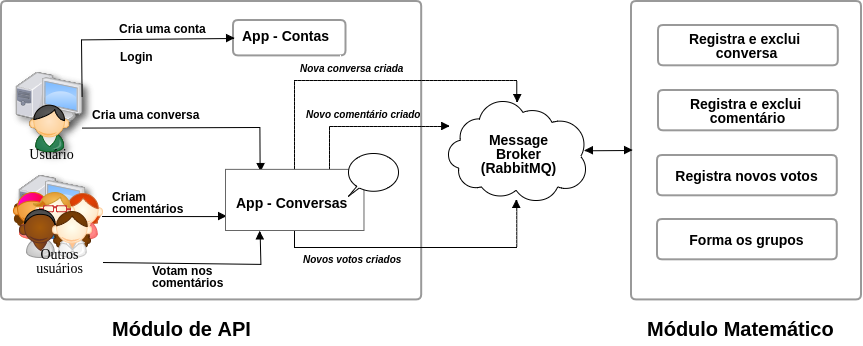
\includegraphics[scale=0.5]{figuras/resumo_ej_api.png}
	\caption{Funcionamento do Empurrando Juntos - Comunicação entre os módulos}
	\label{fig:resumo_ej_api}
	\end{figure}


	Na Figura \ref{fig:resumo_ej_api} é apresentado o fluxo de funcionamento do Empurrando Juntos de acordo com a arquitetura
	estabelecida e a API desenvolvida neste trabalho.
	
	Inicialmente, um usuário faz o cadastro e/ou autentica na aplicação,
	cuja requisição é tratada pelo \textit{app} de contas.
	Após a autenticação do usuário, ele pode criar conversas e comentários na aplicação.
	Outros usuários podem criar comentários e votar nos comentários.
	Todas essas operações relacionadas à conversas, comentários e votos
	são tratadas pelo \textit{app} de conversas.
	Quando uma nova conversa é criada, um novo comentário ou um novo voto é realizado
	em algum comentário de uma conversa, um sinal é disparado pelo \textit{app} de conversas
	para informar o ocorrido ao módulo matemático, enfileirando a tarefa correspondente
	no \textit{message broker}, via Celery.
	Essa chamada é recebida pelo \textit{message broker} que por sua vez delega
	a tarefa ao Celery do módulo matemático.
	Quando o número de votos configurado no sistema é atingido o \textit{app} de conversas
	faz uma chamada para a tarefa de clusterização que, ao ser recebida pelo módulo matemático,
	é a tarefa responsável por calcular os \textit{clusters} considerando o usuário do novo voto,
	gerando e retornando os novos grupos de usuários. Esse número de votos configurado é responsabilidade
	da implementação do módulo para poder gerenciar os momentos em que deve ser realizada clusterização visando 
	uma boa performance da aplicação.
	
	Com o intuito de validar a implementação dessa API foram implementados os outros módulos estabelecidos na arquitetura da
	solução, apresentada na Figura \ref{fig:pentano}. A descrição destes dois módulos e da validação será apresentada no próximo
	capítulo.
	
	